%
% Tutorial -- Active Filters Design with Qucs and Qucsactivefilter
%
% Copyright (C)  2014 Vadim Kuznetsov
%
% Permission is granted to copy, distribute and/or modify this document
% under the terms of the GNU Free Documentation License, Version 1.1
% or any later version published by the Free Software Foundation.
%


\usetikzlibrary{patterns}
\usetikzlibrary{circuits}
\usetikzlibrary{circuits.ee}
\usetikzlibrary{circuits.ee.IEC}
\usetikzlibrary{circuits.logic.IEC}
\usetikzlibrary{intersections}

\tableofcontents

\chapter{Introduction}

The purpose of this report is description of background mathematics used in
Qucsactivefilter.

Qucsactivefilter is powerful active filter design tool. It could be called from
\emph{Tools->Active Filters} menu. It allows you to build active filter circuit
and simulate it with Qucs. Qucsactivefilter builds active filters circuits based
on RC-components and operational amplifier (opamp). 


It is need to define following four groups of parameters to calculate active
filter:

\begin{enumerate}
 \item Frequency response approximation type. Butterworth, Chebyshev,
Inverse Chebyshev,  Cauer (Elliptic) and Bessel filters are available.
 \item Frequency response parameters: filter gain and bandwidth.
 \item Filter topology. Sallen-Key, Mutifeedback (MFB) and Cauer topologies are
available.
 \item Filter type. Low-pass, high-pass, band-pass and band-stop filters are
available.
\end{enumerate}

Filter synthesis method used by Qucsactivefilter is based on filter transfer
function poles and zeros analysis in frequency domain.

\chapter{Filter transfer function}

\section{Frequency domain filter response}

There are 4 main types frequency domain filter responses:

\begin{enumerate}
 \item Low-pass filter (LPF)
 \item High-pass filter (HPF)
 \item Band-pass filter (BPF)
 \item Band-stop filter (BSF)
\end{enumerate}

Magnitude responses $|H(j\omega)|$ of ideal filters are shown in the Figure
\ref{fig:ideal}. 

\begin{figure}[!ht]
\centering
\begin{tikzpicture}
\begin{scope}[xshift=0mm]
\draw [-latex] (0,0) -- (4,0) node [anchor=west] {$\omega$};
\draw [-latex] (0,0) -- (0,2) node [anchor=south] {$|H(j\omega)|$};
\draw [very thick] (0,1.5) -| (2.5,0) node [anchor=north] {$\omega_c$};
\node at (2,-1) {LPF};
\end{scope}
\begin{scope}[xshift=60mm]
\draw [-latex] (0,0) -- (4,0) node [anchor=west] {$\omega$};
\draw [-latex] (0,0) -- (0,2) node [anchor=south] {$|H(j\omega)|$};
\draw [very thick] (1.5,0) node [anchor=north] {$\omega_c$} |- (3.5,1.5);
\node at (2,-1) {HPF};
\end{scope}
\begin{scope}[xshift=0mm,yshift=-40mm]
\draw [-latex] (0,0) -- (4,0) node [anchor=west] {$\omega$};
\draw [-latex] (0,0) -- (0,2) node [anchor=south] {$|H(j\omega)|$};
\draw [very thick] (1.5,0) node [anchor=north] {$\omega_{p1}$} |- ++(1,1.5) -- 
      ++(0,-1.5) node [anchor=north] {$\omega_{p2}$};
\node at (2,-1) {BPF};
\end{scope}
\begin{scope}[xshift=60mm,yshift=-40mm]
\draw [-latex] (0,0) -- (4,0) node [anchor=west] {$\omega$};
\draw [-latex] (0,0) -- (0,2) node [anchor=south] {$|H(j\omega)|$};
\draw [very thick] (0,1.5) -| (1.5,0) node [anchor=north] {$\omega_{s1}$};
\draw (2.5,0) node [anchor=north] {$\omega_{s2}$} |- (3.5,1.5)  ;
\node at (2,-1) {BSF};
\end{scope}
\end{tikzpicture}
\caption{Magnitude responses of ideal filters} \label{fig:ideal}
\end{figure}

By $\omega_c$ denote the \emph{cutoff frequency} of the filter. LPF passes all
frequencies below $\omega_c$ and rejects all frequencies upper $\omega_c$. HPF
operates contrariwise. Magnitude responses  of ideal filters have rectangular form.
Magnitude responses of physical filters have smoothed curves form. Frequency response of 
HPF,BPF and BSF could be normalized to low-pass
prototype. For this reason we consider low-pass active filter further. It will
be shown how to transform HPF, BPF, and BSF to low-pass prototype filter.

\section{Transfer function general form}

Active filters are characterized by transfer function in frequency domain.
Common form of the filter transfer function is given here:

\begin{equation}
 H(s)=\frac{b_m s^m+b_{m-1}s^{m-1}+\ldots+b_2 s^2+b_1 s+b_0}
           {a_n s^n+a^{n-1}s^{n-1}+\ldots+a_2 s^2+a_1 s+a_0} \label{trfunc}
\end{equation}

The filter order $N$ is:

\begin{equation}
 N = \max(m,n)
\end{equation}

Filter order determines the number of filter sections and filter circuit
complexity. Active filter consists of $k=\lfloor N/2\rfloor$ 2-nd order section
and $k=\lceil N \mod 2 \rceil$ 1-st order sections. 

Zeros of the transfer function are the roots of numerator.  Poles are the roots
of denominator. We need to know filter transfer function to determine components
(resistors and capacitors --- RC) values of the active filter circuit.

We can obtain magnitude $A(\omega)$ and phase $\theta(\omega)$ responses  using
transfer function:

\begin{equation}
 A(\omega)=|H(j\omega)|
\end{equation}
\begin{equation}
 \theta(\omega)=\arg(H(j\omega))
\end{equation}



Qucsactivefilter uses filter design algorithms provided by \cite{johnson}.

\section{Poles and Zeros}

Transfer function could be represented as a ratio of numerator $P(s)$ and
denominator $Q(s)$ polynomials. Each of these polynomials could be factorized:
\begin{equation}
 H(s)=\frac{P(s)}{Q(s)}=H_0\frac{(s-z_1)(s-z_2)(s-z_3)\ldots(s-z_m)}
                                {(s-p_1)(s-p_2)(s-p_3)\ldots(s-p_n)}
\end{equation}

The roots of the numerator $z_1,z_2,z_3,\ldots,z_m$ are called zeros of the
transfer function. The roots of the denominator $p_1,p_2,p_3,\ldots,p_n$ are
called poles of the transfer function. The $n$-th order polynomial has $n$
roots. $H_0$ is DC gain of the filter.

If $P(s)$ and $Q(s)$ are polynomials with real coefficients, each pole or zero
has its complex-conjugated pair. For example for $n$-th order:

\begin{equation}
 p_{i}=p_{n-i} = \sigma_{pi}\pm j\omega_{pi} \label{pole}
\end{equation}
\begin{equation}
 z_{i}=z_{n-i} = \sigma_{zi}\pm j\omega_{zi} \label{zero}
\end{equation}

$\sigma_i$ is real part of the pole or zero: 

\begin{equation}
\sigma_{pi}=\Re[p_i]\qquad\omega_{pi}=\Im[p_i] 
\end{equation}

$\omega_i$ is imaginary part of the pole or zero:

\begin{equation}
\sigma_{zi}=\Re[z_i]\qquad\omega_{zi}=\Im[z_i]
\end{equation}

\section{Time domain parameters}

\emph The {impulse response} $h(t)$ is the filter output signal when \emph{Dirac
delta impulse} is applied to its input. Impulse response is inverse Laplace
transform of the filter transfer function:

\begin{equation}
 h(t)=\mathcal{L}^{-1}[H(s)]
\end{equation}

\emph The {step response} $g(t)$ is the filter output signal when \emph{unit
step} is applied to filter input. Step response could be expressed via inverse
Laplace transform:

\begin{equation}
 g(t)=\mathcal{L}^{-1}\left[\frac{H(s)}{s}\right]
\end{equation}

Impulse response is derivative of step response
\begin{equation}
 h(t)=\frac{d}{dt}g(t)
\end{equation}

The \emph{phase delay} $\tau_p(\omega)$ of a system is defined using phase
response $\theta(\omega)$

\begin{equation}
 \tau_p(\omega)=\frac{-\theta(\omega)}{\omega} \label{eq:ph_delay}
\end{equation}

Phase delay is time delay of the sinusoidal signal of frequency $\omega$
passing through the filter.

The \emph{group delay} is defined as
\begin{equation}
 \tau_g (\omega)= -\frac{d}{dt}\theta(\omega)
\end{equation}

The group delay is the measure of modulated signal distortion. Group delay is
important for high-quality audio signals amplification.




\section{Transfer function approximations}


Magnitude and phase response type depends on transfer function numerator and
denominator polynomials coefficients $a_i$ and $b_i$. Substituting different
sets of $a_i$ and $b_i$ we can implement different filters: low-pass, high-pass,
band-pass and band-stop. The following polynomials are the most frequently
used for the active filters design purposes :

\begin{enumerate}
 \item Butterworth
 \item Chebyshev --- Type I
 \item Chebyshev --- Type II (Inverse Chebyshev)
 \item Cauer
 \item Bessel
 \item Legendre
\end{enumerate}

Polynomials coefficients are calculated using filter approximation.
Every transfer function approximation has its own set of poles and zeros. It is
need to note that Butterworth, Chebyshev Type I and Bessel filters have no
zeros. 

\verb|Qucsactivefilter| evaluates poles and zeros for given approximation and
then evaluates RC-elements values for each section of active filter.

You can define $a_i$ and $b_i$ coefficients of the transfer function
(\ref{trfunc}) manually with \verb|Qucsactivefilter|. This method is
suitable for unknown or new approximation. Then \verb|Qucsactivefilter|
evaluates poles and zeros and builds filter circuit. See
\verb|Filter::calcUserTrFunc()| in \verb|filter.cpp| for details.

\section{Physical active filter transfer function}

Physical active filter of $N$-th order consists of $N_{2} = \lfloor N/2\rfloor$
2-nd order sections and $N\mod 2$ 1-st order sections. Physical filter consists
of
\begin{equation}
 N_{sec}=\lfloor N/2\rfloor+N\mod 2 \label{order-sections}
\end{equation}
total 2-nd order nad 1-st order sections.

So, transfer function can be represented as product of the each filter section
transfer functions.

For $i$-th 2-nd order section which have transfer function zeros (Cauer and
Chebyshev Type II) we have following section transfer function:

\begin{equation}
 H_2(s)=H_0^1\frac{s^2+A_i\omega_c^2}{s^2+B_i\omega_c s+C_i\omega_c^2}
\label{2ord1}
\end{equation}

And for $i$-th 2-nd order section without zeros (Butterworth, Chebyshev Type I)
and Bessel:
\begin{equation}
 H_2(s)=H_0^1\frac{C_i\omega_c^2}{s^2+B_i\omega_c s+C_i\omega_c^2} \label{2ord2}
\end{equation}

For $N-th$ 1-st order section:
\begin{equation}
 H_1(s)=\frac{H_0^1}{s+C_N\omega_c} \label{1ord}
\end{equation}


where $A$, $B$, $C$ --- are determined by poles and zeros location; $\omega_c$
is filter cutoff frequency.

$H_0^1$ is DC gain of the $i$-th section:

\begin{equation}
 H_0^1 = (H_0)^{1/N_{sec}} 
\end{equation}

Let's consider normalized form of the filter frequency response.
For normalized frequency response we assume $\omega_c=1$.

Common form of the filter transfer function could be factorized as below. For
odd order filters without transfer function zeros (Butterworth, Chebyshev Type-I
and Bessel):

\begin{equation}
 H(s)=H_1(s)\prod_{i=0}^{N_2}H_2(s) = 
 H_0\frac{1}{s+C_N}\prod_{i=0}^{N_2}\frac{C_i}{s^2+B_i s+C_i}
\end{equation}

For odd order filter with transfer function zeros (Cauer and Chebyshev-Type-II)

\begin{equation}
 H(s)=H_1(s)\prod_{i=0}^{N_2}H_2(s) = 
 H_0\frac{1}{s+C_N}\prod_{i=0}^{N_2}\frac{s^2+A_i}{s^2+B_i s+C_i}
\label{trfunc-quad}
\end{equation}

For even order filter without transfer function zeros:

\begin{equation}
 H(s)=\prod_{i=0}^{N_2}H_2(s) = H_0\prod_{i=0}^{N_2}\frac{C_i}{s^2+B_i
s+C_i}
\end{equation}

For even order filter with transfer function zeros:
\begin{equation}
 H(s)=\prod_{i=0}^{N_2}H_2(s) = 
 H_0\prod_{i=0}^{N_2}\frac{s^2+A_i}{s^2+B_i s+C_i}
\end{equation}

Every 2-nd order factor matches one pair of complex conjugated poles and one
pair of complex conjugated zeros. First-order factor matches one real pole.

Filter synthesis method proposed in this paper uses $A_i$, $B_i$, $C_i$
coefficients to evaluate active filter RC-elements values. We should find
$A_i$, $B_i$, $C_i$ coefficients using poles and zeros location to find
RC-elements values.

\section{Physical active filter poles and zeros}

Even $N$-th order physical active filter transfer function has no zeros or $N/2$
complex conjugated pairs of zeros and $N/2$ complex conjugated pairs of poles.
Odd order physical active filter transfer function has additional real pole.

We need to solve numerator of $i$-th factor (\ref{2ord1}) equals zeros to find
$i$=th zero pair location:

\begin{equation}
 s^2+A_i=0
\end{equation}

\begin{equation}
 z_{i,N-i}=\pm j\sqrt{A_i}
\end{equation}

And we can find coefficient $A_i$ by known $i$-th zero pair imaginary part
\ref{zero}:
\begin{equation}
 z_{i,N-i}=\pm j\omega_{zi}
\end{equation}
\begin{equation}
 A_i=\omega_{zi}^2 \label{Ai}
\end{equation}

Zeros of the physical active filter transfer function have no real part.
Using this equation (\ref{Ai})we can find $A_i$ coefficients by known zeros
location. Zeros location (and real and imaginary part) could be found using
transfer function approximation (Butterworth, Chebyshev, etc.).

We need to solve the following quadratic equation to find $i$-th pole location
(denominator of $i$-th 2-nd order factor equals zero):
\begin{equation}
 s^2+B_is + C_i = 0
\end{equation}

Solution of this equation yields complex conjugated pair of poles:
\begin{equation}
 p_{i,N-i}=\sigma_{pi}\pm
j\omega_{pi}=-\frac{B_i}{2}\pm\frac{\sqrt{-B_i^2+4C_i}}{2}
\label{pole_from_quad}
\end{equation}

We need to solve the next system of equations find $B_i$ and $C_i$ by known
poles location:
\begin{equation}
 \omega_{pi}=\frac{\sqrt{-B_i^2+4C_i}}{2}
\end{equation}
\begin{equation}
 \sigma_{pi}=-\frac{B_i}{2}
\end{equation}

Solution of this system yields:
\begin{equation}
 B_i=-2\sigma_{pi} \label{Bi}
\end{equation}
\begin{equation}
 C_i=\sigma_{pi}^2+\omega_{pi}^2 \label{Ci}
\end{equation}

Odd order $N$-th filters have one $N$-th real pole $p_N=\sigma_{N}\pm j\cdot0$.
To find this pole we need to solve the following equation (denominator of the
(\ref{1ord}) equals zero):
\begin{equation}
 s+C_N=0
\end{equation}

Solution gives:
\begin{equation}
 p_N =\sigma_N = -C_N
\end{equation}

And we can find $C_N$ coefficient by known real part of $N-th$ real pole:
\begin{equation}
 C_N=-\sigma_N \label{CN-1ord}
\end{equation}

Using poles and zeros location and equation (\ref{Ai}, (\ref{Bi}) and
(\ref{Ci}) we can find $A_i$, $B_i$, $C_i$ coefficients, factorize transfer
function to (\ref{trfunc-quad}) form and find filter RC-elements values.

\chapter{Low-pass filters transfer function approximations}

\section{Butterworth}

\subsection{Transfer function}

Butterworth filter implements magnitude response as flat as possible in pass
band. Magnitude response monolitically decays outside passband.

Normalized magnitude response of $N$-th order the Butterworth filter has the
form:
\begin{equation}
 |H(j\omega)|=\sqrt{\frac{1}{1+(\omega/\omega_c)^{2N}}}
\end{equation}

\begin{figure}[!ht]
  \centering
  \begin{tikzpicture}
   \draw[-latex] (0,0) -- (7,0) node [anchor=west] {$\omega$};
   \draw[-latex] (0,0) -- (0,5) node [anchor=south]
    {$|H(j\omega)|$};
%      \draw [ y=4cm, x=3cm,,smooth,name path=MR,
%      declare function={K(\w)=1/((1+\w^8.0)^0.5);}] plot [domain=0:2]
%  (\x,{K(\x)});
     \draw[domain=0:2,y=4cm, x=3cm,smooth,name path=MR] plot
           function{1/(1+x**8)**0.5};
    \path [name path=Fc] (0,3.5) -- (5,3.5);
    \path [name path=Fs] (0,1) -- (5,1);
    \draw [dashed,name intersections={of=MR and Fc}] (0,3.5) node [anchor=east]
    {$\alpha_p$} -- (intersection-1);
    \draw [dashed,name intersections={of=MR and Fc}] (intersection-1) |- (0,0);
    \draw [dashed,name intersections={of=MR and Fs}] (0,1) node [anchor=east]
    {$\alpha_s$} -- (intersection-1);
    \draw [dashed,name intersections={of=MR and Fs}] (intersection-1) |- (0,0);
    \node [anchor=north] at (2.6,0) {$\omega_c$};
    \node [anchor=north] at (4.2,0) {$\omega_s$};
  \end{tikzpicture}
  \caption{Typical 4-th order Butterworth filter magnitude response}
  \label{fig:butterw}
\end{figure}
% \FloatBarrier

Transfer function of $N$-th order Butterworth filter could be factorized as
following:

\begin{equation}
 H(s) = \frac{1}{\prod\limits_{i=1}^N(s-p_i)}=
\frac{1}{(s-p_1)(s-p_2)\ldots(s-p_N)}
\end{equation}

where $p_i$ are transfer function poles. Butterworth filter has no zeros. Poles
location could be determined as following \cite{Hamming}:

\begin{equation}
 p_i = e^{j\pi[(2i+N-1)/2N]} = 
 \cos\left(\frac{2i+N-1}{2N}\right) + j\sin\left(\frac{2i+N-1}{2N}\right)
\label{butt-poles}
\end{equation}

\verb|Filter::calcButterworth()| function implements such poles location
evaluation according equation (\ref{butt-poles}). For sources see
\verb|filter.cpp|.


\subsection{Minimun order estimation}

We need to know maximum passband attenuation $A_p$ and minimum stopband
attenuation $A_s$ to estimate minimum Butterworth order. These attenuations
often are measured in decibels (dB).

These values are determined by absolute attenuation $\alpha_p$ at cutoff
frequency $\omega_c$ and attenuation $\alpha_s$ at stopband frequency
$\omega_s$.

\begin{equation}
 A_p = 20\log\alpha_p
\end{equation}

\begin{equation}
 A_s = 20\log\alpha_s
\end{equation}



The next equation determines the minimum order of the Butterworth filter.

\begin{equation}
 N = \frac{1}{2\log(\omega_s/\omega_c)} \cdot
\frac{\log(10^{0.1A_s}-1)}{\log(10^{0.1A_p}-1) } \label{butt-order}
\end{equation}

This filter has $A_p$ attenuation value at cutoff frequency $\omega_c$
and at least $A_s$ attenuation at stopband frequency $\omega_s$.


\section{Chebyshev Type-I}

\subsection{Transfer function}

Chebyshev filters provide more sufficient more sharp transition from pass band
to stop band than Butterworth filter. But it has ripple in passband $R_p$ up to
3dB.
Passband magnitude response of the Chebyshev filter is not flat. 

Magnitude response of the $N-th$ order Chebyshev Type-I filter is determined by
equation:

\begin{equation}
 H(j\omega) = \frac{1}{\sqrt{1+\varepsilon^2 T^2_N(\omega/\omega_c)}}
\end{equation}

where $T^2_N(\omega)$ is $N$-th order Chebyshev polynomial.

\begin{equation}
 T^2_N(x) = \cos(N\arccos(x)) \label{cheb-poly}
\end{equation}

$\varepsilon$ is the ripple coefficient:

\begin{equation}
 \varepsilon = \sqrt{10^{0.1R_p}-1} \label{eps}
\end{equation}

For $R_p$=3dB we obtain $\varepsilon=1$. For $R_p$=0dB (no ripple) we obtain
$\varepsilon=0$. 


\begin{figure}[!ht]
  \centering
  \begin{tikzpicture}
   \draw[-latex] (0,0) -- (7,0) node [anchor=west] {$\omega$};
   \draw[-latex] (0,0) -- (0,5) node [anchor=south]
    {$|H(j\omega)|$};
%     \draw [very thick, y=4cm, x=3cm,
%     declare function={K(\w)=1/((1+\w^8.0)^0.5);}] plot [domain=0:2]
% (\x,{K(\x)});
    \draw[domain=0:2,y=4cm, x=3cm,samples=200,name path=MR,smooth] plot
          function{1/(sqrt(1+0.5**2*((cos(4*acos(x)))**2)))};
    \path [name path=Fc] (0,3.5) -- (5,3.5);
    \path [name path=Fs] (0,1) -- (5,1);
    \draw [dashed,name intersections={of=MR and Fc}] (0,3.5) node [anchor=east]
    {$\alpha_p$} -- (intersection-1);
    \draw [dashed,name intersections={of=MR and Fc}] (intersection-1) |- (0,0);
    \draw [dashed,name intersections={of=MR and Fs}] (0,1) node [anchor=east]
    {$\alpha_s$} -- (intersection-1);
    \draw [dashed,name intersections={of=MR and Fs}] (intersection-1) |- (0,0);
    \node [anchor=north] at (2.6,0) {$\omega_p$};
    \node [anchor=north] at (4.2,0) {$\omega_s$};
  \end{tikzpicture}
  \caption{Typical 4-th order Chebyshev filter magnitude response}
  \label{fig:cheb}
\end{figure}

The poles $p_i$ of the Chebyshev Type-I filter could be evaluated as following 
\cite{Hamming}. The poles are the roots of the $N$-th order Chebyshev 
polynomial:

\begin{equation}
 p_i = \sigma_i + j\omega_i
\end{equation}

\begin{equation}
 \sigma_i = -\sin\left(\frac{(2i-1)\pi}{2N}\right)           
\sinh\left[\frac{1}{N}\sinh^{-1}\left(\frac{1}{\varepsilon}\right)\right]
\label{pol-cheb1}
\end{equation}

\begin{equation}
 \omega_i = \cos\left(\frac{(2i-1)\pi}{2N}\right)           
\cosh\left[\frac{1}{N}\sinh^{-1}\left(\frac{1}{\varepsilon}\right)\right]
\label{pol-cheb2}
\end{equation}

Chebyshev filters have no zeros. We should know filter order $N$ and acceptable
bandpass ripple $R_p$ to find filter poles. \verb|Filter::calcChebyshev|
function evaluates Chebyshev filter poles using equations (\ref{pol-cheb1}) and
(\ref{pol-cheb2}) (see \verb|filter.cpp|).

\subsection{Minimun order estimation}

The minimum order $N$ of the Chebyshev filter can be estimated using following
equation. We assume $A_p=R_p$.

\begin{equation}
 N = \frac{\cosh^{-1}(\sqrt{(10^{0.1A_s}-1)/\varepsilon^2})} 
          {\cosh^{-1}(\omega_s/\omega_c)} \label{cheby1-order}
\end{equation}

where $\varepsilon$ could be evaluated from equation (\ref{eps}). It's need to
know stopband attenuation $A_s$ (dB), passband ripple $R_p$ (dB), cutoff
frequency $\omega_c$, and stopband frequency $\omega_s$.
\verb|Filter::calcChebyshev()| function performs such estimation. See
\verb|filter.cpp| for source code.

Chebyshev Type-I and Butterworth filters are the most frequently used ones.

\section{Chebyshev Type-II}

\subsection{Transfer function}

Magnitude response of the $N-th$ order Chebyshev Type-I (or inverse Chebyshev)
filter is determined by equation:

\begin{equation}
 H(j\omega) = \frac{1}{\sqrt{1+\dfrac{1}{\varepsilon^2
T^2_N(\omega_c/\omega)}}}
\end{equation}

where $T_N(\omega)$ is Chebyshev polynomial (\ref{cheb-poly}).

Stopband ripple $R_s$ is determined by $\varepsilon$
\begin{equation}
 \varepsilon = \frac{1}{\sqrt{10^{0.1R_s}-1}}
\end{equation}

Typical magnitude response of the 4-th order Chebyshev Type-II filter is shown
in the Figure \ref{fig:cheb2}.

\begin{figure}[!ht]
  \centering
  \begin{tikzpicture}
   \draw[-latex] (0,0) -- (7,0) node [anchor=west] {$\omega$};
   \draw[-latex] (0,0) -- (0,5) node [anchor=south]
    {$|H(j\omega)|$};
%     \draw [very thick, y=4cm, x=3cm,
%     declare function={K(\w)=1/((1+\w^8.0)^0.5);}] plot [domain=0:2]
% (\x,{K(\x)});
    \draw[domain=0:2,y=4cm, x=3cm,samples=200,name path=MR] plot
function{1/(sqrt(1+1/(0.25**2*((cos(4*acos(1/x)))**2))))};
    \path [name path=Fc] (0,3.5) -- (5,3.5);
    \path [name path=Fs] (0,1) -- (5,1);
    \draw [dashed,name intersections={of=MR and Fc}] (0,3.5) node [anchor=east]
    {$\alpha_p$} -- (intersection-1);
    \draw [dashed,name intersections={of=MR and Fc}] (intersection-1) |- (0,0);
    \draw [dashed,name intersections={of=MR and Fs}] (0,1) node [anchor=east]
    {$\alpha_s$} -- (intersection-1);
    \draw [dashed,name intersections={of=MR and Fs}] (intersection-1) |- (0,0);
    \node [anchor=north] at (2.6,0) {$\omega_p$};
    \node [anchor=north] at (4.2,0) {$\omega_s$};
  \end{tikzpicture}
  \caption{Typical 4-th order Chebyshev Type-II filter magnitude response}
  \label{fig:cheb2}
\end{figure}

You can see from this figure that this filter has flat response at passband and
ripple at stopband.

$N$-th order Chebyshev Type-II filter has $N$ imaginary zeros. The location of
the $i$-th zero $z_i$ could be estimated using following equations:
\begin{equation}
 z_i = j\omega_{zi}
\end{equation}
\begin{equation}
 \omega_{zi} = -\frac{1}{\cos\left(\dfrac{(2i-1)\pi}{2N}\right)}
\end{equation}

Also $N$-th order Chebyshev Type-II filter has $N$ imaginary poles. The
location of the $i$-th pole $p_i$ is determined by following equations. The
poles are inverse to poles of the Chebyshev Type-I filter. And Chebyshev
Type-II filters are known as inverse Chebyshev filters.

\begin{equation}
 p_{i} = \frac{1}{\sigma_{pi}+j\omega_{pi}}
\end{equation}
\begin{equation}
 \sigma_{pi} = -\sin\left(\frac{(2i-1)\pi}{2N}\right)           
\sinh\left[\frac{1}{N}\sinh^{-1}\left(\frac{1}{\varepsilon}\right)\right]
\end{equation}

\begin{equation}
 \omega_{pi} = \cos\left(\frac{(2i-1)\pi}{2N}\right)           
\cosh\left[\frac{1}{N}\sinh^{-1}\left(\frac{1}{\varepsilon}\right)\right]
\end{equation}

\subsection{Minimun order estimation}

The minimum order $N$ of the Chebyshev filter can be estimated using following
equation. We assume $A_s=R_s$.

\begin{equation}
 N = \frac{\cosh^{-1}(\sqrt{(10^{0.1A_s}-1)})}{\cosh^{-1}(\omega_s/\omega_c)}
\label{cheby2-order}
\end{equation}

It's need to
know stopband attenuation $A_s$ (dB), passband ripple $R_p$ (dB), cutoff
frequency $\omega_c$, and stopband frequency $\omega_s$.
\verb|Filter::calcInvChebyshev()| function performs such estimation. See
\verb|filter.cpp| for source code.

\section{Cauer (Elliptic)}

\subsection{Transfer function and magnitude response}

Cauer or Elliptic filters have ripple in pass band and in stop band. These
filters have the sharpest magnitude frequency response. Magnitude response is
determined by following equation:

\begin{equation}
 |H(j\omega)|=\frac{1}{\sqrt{1+\varepsilon^2 R^2_N(\omega/\omega_c,L)}}
\end{equation}

where $R_N(\omega,L)$ is $N$-th order elliptic rational function with ripple
parameter $L$.

Typical magnitude response is shown in the Figure \ref{fig:cauer}.

\begin{figure}[!ht]
  \centering
  \begin{tikzpicture}
   \draw[-latex] (0,0) -- (7,0) node [anchor=west] {$\omega$};
   \draw[-latex] (0,0) -- (0,5) node [anchor=south]
    {$|H(j\omega)|$};
%     \draw [very thick, y=4cm, x=3cm,
%     declare function={K(\w)=1/((1+\w^8.0)^0.5);}] plot [domain=0:2]
% (\x,{K(\x)});
    \draw[domain=0:2,y=4cm, x=3cm,samples=200,name path=MR] plot function{1/((0.25*((1.846*(1.305*x**2-1)**2)/(1-0.695*x**2)**2-1)**2)/(1-(.153*(1.305*x**2-1)**2)/(1-0.695*x**2)**2)**2+1)**0.5};
    \path [name path=Fc] (0,3.5) -- (5,3.5);
    \path [name path=Fs] (0,1) -- (5,1);
    \draw [dashed,name intersections={of=MR and Fc}] (0,3.5) node [anchor=east]
    {$\alpha_p$} -- (intersection-1);
    \draw [dashed,name intersections={of=MR and Fc}] (intersection-1) |- (0,0);
    \draw [dashed,name intersections={of=MR and Fs}] (0,1) node [anchor=east]
    {$\alpha_s$} -- (intersection-1);
    \draw [dashed,name intersections={of=MR and Fs}] (intersection-1) |- (0,0);
    \node [anchor=north] at (2.6,0) {$\omega_p$};
    \node [anchor=north] at (4.2,0) {$\omega_s$};
  \end{tikzpicture}
  \caption{Typical 4-th order Cauer(Elliptic) filter magnitude response}
  \label{fig:cauer}
\end{figure}

You can see from this figure that Cauer filter has the most sharpest magnitude
response. But this filter has both bandpass ripple and bandstop ripple. 

\subsection{Minimun order estimation}

We need to know cutoff frequency $\omega_c$, stopband frequency $\omega_s$,
passband ripple $R_p$, stopband attenuation $A_s$. We assume $A_p=R_p$ and
$R_s=A_s$. Minimum order estimation method follows Handbook
\cite{dfd_handbook}, page 95.

Minimun filter order could be estimated using following steps:

\begin{enumerate}
 \item Determine selectivity factor $k$
 \begin{equation}
  k = \omega_c/\omega_s \label{k_cauer}
 \end{equation}
 \item Compute the modular constant $q$
 \begin{equation}
  q = u +2u^5+15u^9+150u^{13} \label{q_cauer}
 \end{equation}
 \begin{equation}
  u = \frac{1-\sqrt[4]{1-k^2}}{2(1+\sqrt[4]{1-k^2})}
 \end{equation}
\item Compute the discrimination factor $D$
\begin{equation}
 D = \frac{10^{0.1A_s}-1}{10^{0.1A_p-1}}
\end{equation}
\item Estimate the minimum required order of the Cauer filter
\begin{equation}
 N = \left\lceil\frac{\log 16D}{\log(1/q)}\right\rceil \label{cauer-order}
\end{equation}

\end{enumerate}

\verb|Filter::cauerOrderEstim()| function implements this algorithm. See
\verb|filter.cpp|.

\subsection{Poles and zeros}

Elliptic rational functions are expressed via Jacobi elliptic cosine functions.
By this reason you should use polynomial approximations to find poles and zeros
of the transfer function. Qucsactivefilter uses algorithm based on 
\emph{Digital Filter Designer's Handbook} \cite{dfd_handbook}.

This algorithm consists of three steps:
\begin{enumerate}
 \item Estimate the minimum order of the Cauer filter using magnitude
response parameters
 \item Evaluate coefficients $A_i$, $B_i$, $C_i$ for transfer function
factorization (\ref{trfunc-quad}) using algorithm from pages 95
-- 97 of the Handbook \cite{dfd_handbook}.
 \item Find poles and zeros as roots of quadratic equation using equations
(\ref{pole_from_quad}) and (\ref{Ai}). You also need to find $N$-th real pole
$p_N$ for odd filter order.
\end{enumerate}

Use following steps to calculate $A_i$, $B_i$, $C_i$ coefficient for every
section of the $N$-th order Cauer filter.

\begin{enumerate}
 \item Determine selectivity factor $k$ (\ref{k_cauer}) and modular constant $q$
(\ref{q_cauer})
\item Compute $V$ as
\begin{equation}
 V=\frac{1}{2N}\ln\left(\frac{10^{A_p/20}+1}{10^{A_p/20}-1}\right)
\end{equation}
\item Compute $p_0$ as
\begin{equation}
 p_0=\left|
     \frac{q^{1/4}\sum\limits_{m=0}^{\infty}(-1)^m q^{m(m+1)}\sinh[(2m+1)V]}
     {0.5+\sum\limits_{m=0}^{\infty}(-1)^m q^{m^2}\cosh(2mV)}\right|
\end{equation}
\item Compute $W$ as
\begin{equation}
 W=\left[\left(1+\frac{p^2_0}{k}\right)(1+k p_0^2)\right]^{1/2}
\end{equation}
\item Determine the number $r$ of 2-nd order sections
\begin{equation}
 r = \lfloor \frac{N}{2} \rfloor
\end{equation}
\item For each $i$-th 2-nd order section $i=1,2,\ldots,r$ compute $X_i$ as
\begin{equation}
 X_i=\frac{2q^{1/4}\sum\limits_{m=0}^{\infty}(-1)^m
     q^{m(m+1)}\sin[(2m+1)\mu\pi V/N]}
     {1+2\sum\limits_{m=0}^{\infty}(-1)^m q^{m^2}\cos(2m\mu\pi/N)}
\end{equation}
where 
\begin{equation}
 \mu=\left\lbrace \begin{array}{ll}
i, & \quad N \mbox{ odd} \\
i-1/2, & \quad N \mbox{ even} 
\end{array} \right.
\end{equation}
\item For each $i$-th 2-nd order section $i=1,2,\ldots,r$ compute $Y_i$ as
\begin{equation}
 Y_i=\left[\left(1-\frac{X_i^2}{k}\right)(1-kX_i^2)\right]
\end{equation}

\item Compute coefficients $A_i$, $B_i$, $C_i$ using $W$, $X_i$, $Y_i$
\begin{equation}
 A_i=\frac{1}{X_i^2}
\end{equation}
\begin{equation}
 B_i=\frac{2p_0Y_i}{1+p_0^2X_i^2}
\end{equation}
\begin{equation}
 C_i=\frac{(p_0Y_i)^2+(X_iW)^2}{(1+p_0^2X_i^2)^2}
\end{equation}

\item For odd filter order compute $N$-th real pole $p_N$
\begin{equation}
 p_N=-p_0
\end{equation}
\end{enumerate}

\verb|Filter::cauerOrderEstim()| and \verb|Filter::calcCauer()| implement this
algorithm. These functions are called together. See \verb|filter.cpp|.

\section{Bessel}

For all considered filter transfer approximations magnitude response was 
considered. Phase response was not taken into account. Bessel filter belongs to 
filtes with normalized phase delay $\tau_p$ (\ref{eq:ph_delay}). Phase response 
of such filter is linear-dependent on frequency

\begin{equation}
 \theta(\omega) = -\omega \tau_p
\end{equation}

Phase response of Bessel filters approaches to such dependency in some 
frequency range.

Transfer function of the Bessel filter has following form:
\begin{equation}
 H(s)=\frac{\theta_n(0)}{\theta_n(s/\omega_c)}
\end{equation}

where $\theta_n(s)$ is $n$-th order reverse Bessel polynomial

\begin{equation}
 \theta_n(s)=\sum_{k=0}^{n}a_ks^k
\end{equation}
\begin{equation}
 a_k=\frac{(2n-k)!}{2^{n-k}k!(n-k)!}\qquad k=0,1,\ldots,n
\end{equation}


For example for 5-th order Bessel polynomial:
\begin{equation}
 H(s)=\frac{945}{s^5+15s^4+105s^3+420s^2+945s+945}
\end{equation}

Poles of Bessel transfer function could not be evaluated symbolically. 
Qucs-activefilter uses precalculated poles tables for Bessel filters up to 
20-th order. See header \verb|bessel.h| and Octave script \verb|bessel-poles.m|

Bessel filter transfer function has no zeros. 

Minimal order of the Bessel filter could not be evaluated too. You should 
define it manually. See \verb|Filter::calcBessel()| and \verb|filter.cpp| for 
source code.




% \subsection{Transfer function}

% \subsection{Minimun order estimation}

\chapter{Other filter types}
\label{sec:other-filt}
\section{High-pass filters}

High-pass filters calculation uses low-pass filter prototype. Then you can use
low-pass prototype to determine filter order and poles/zeros.
High-pass transfer function can be transformed to low-pass prototype filter
transfer function.

High-pass filter transfer function $H(s)$ could be mapped to low-pass prototype
filter transfer function $H_{LPF}(s')$. The following transform should be used:

\begin{equation}
 H(s)=H_{LPF}(s')
\end{equation}
\begin{equation}
 s=\frac{1}{s'}
\end{equation}

For cutoff frequency and stopband frequency the following transformations are
valid:

\begin{equation}
 \omega'_c=\frac{1}{\omega_c}
\end{equation}
\begin{equation}
  \omega'_s=\frac{1}{\omega_s}
\end{equation}

We can map cutoff and stopband frequencies of high-pass filter to cutoff
and stopband frequencies of low-pass prototype using these equations. Then we
can use common method of low-pass filters synthesis. We can obtain poles and
zeros of transfer function and determine RC-elements values.



\section{Band-pass filters}

Band-pass filter requires another transformations. 
By $\Omega_0$ denote the center frequency. By $\Delta\Omega$ denote the
bandwidth.

\begin{equation}
 \Omega_0 = \sqrt{\omega_{p1}\omega_{p2}}
\end{equation}
\begin{equation}
 \Delta\Omega = \omega_{p2} - \omega_{p1}
\end{equation}

where $\omega_{p1}$ is lower cutoff frequency; $\omega_{p2}$ is upper cutoff
frequency. Denote by $TW$ transient bandwidth. Upper $\omega_{s2}$ and lower
$\omega_{s1}$ cutoff frequencies are determined as following:
\begin{equation}
 \omega_{s2}=\omega_{p2}-TW
\end{equation}
\begin{equation}
 \omega_{s1}=\omega_{p1}+TW
\end{equation}

Quality factor of band-pass filter is: 
\begin{equation}
 Q=\frac{\Omega_c}{\Delta\Omega}
\end{equation}


We get band-pass filter transfer function:
\begin{equation}
 H(s)=H_{LPF}(s')
\end{equation}
\begin{equation}
 s'=s+\frac{\Omega_0^2}{s}
\end{equation}



Low-pass prototype cutoff frequency $\omega'_c$ and stopband frequency
$\omega'_s$ yield:
\begin{equation}
 \omega'_c = \Delta\Omega
\end{equation}
\begin{equation}
 \omega'_s= \min(|\omega'_{s1}|,|\omega'_{s2}|)
\end{equation}
\begin{equation}
 \omega'_{s1}=\omega_{s1}-\frac{\Omega_0^2}{\omega_{s1}}
\end{equation}
\begin{equation}
 \omega'_{s2}=\omega_{s2}-\frac{\Omega_0^2}{\omega_{s2}}
\end{equation}

Using these equation we can obtain low-pass filter cutoff and stopband
frequencies. Magnitude response ripple parameters are the same. Then we can
obtain filter order and poles/zeros.

Two 2-nd order sections match one complex conjugated pole/zero pair of low-pass
prototype. Band-pass filter has always even order. 




\section{Band-stop filters}

Band stop filters transfer function could be transformed into low-pass filter 
transfer function using the presented substitution. 

\begin{equation}
 H(s)=H_{LPF}(s')
\end{equation}
\begin{equation}
 s'=\dfrac{1}{s+\dfrac{\Omega_0^2}{s}}
\end{equation}

Center frequencies $\Omega_0$ and bandwidth $\Delta\Omega$ are the same as for 
band-pass filter. Cutoff frequency and bandwidth of the low-pass prototype 
could be estimated using approach from the previous section.

\chapter{Filter topologies}

\section{Active filter schematic synthesis algorithm}

Active filter synthesis algorithm contains the following steps. For low-pass
and high-pass filters you can use this algorithm directly without any
adaptations. For band-pass and band-stop filters you should evaluate low-pass
prototype cutoff frequency and stopband frequency first.
\verb|Filter::calcFilter()| function implements these steps. See
\verb|filter.cpp| for sources. Additional information about used filter 
topologies are provided in \cite{johnson,Tiet02,Horowitz}

\begin{itemize}
 \item \textbf{Step 1:} Select desired filter type (low-pass, high-pass,
band-pass, band-stop), filter topology, frequency response approximation type
and following frequency response parameters:
\begin{enumerate}
 \item Cutoff frequency
 \item Stopband frequency
 \item Passband attenuation
 \item Stopband attenuation
 \item Passband ripple (for Chebyshev and Cauer filters only)
 \item Passband gain
\end{enumerate}

\item \textbf{Step 1a:} For all filters except low-pass. Determine cutoff
 frequency, and stopband frequency for low-pass prototype using methods from
section \ref{sec:other-filt}. 

\item \textbf{Step 2:} Estimate filter order $N$ using equation
(\ref{butt-order}) for Butterworth filters, equation (\ref{cheby1-order}) for
Chebyshev Type-I filters, equation (\ref{cheby2-order}) for Chebyshev Type-II
filter, equation (\ref{cauer-order}) for Cauer filter.

\item \textbf{Step 3:} Evaluate poles and zeros of the transfer function using
order value from previous step. Qucsactivefilter stores poles and zeros as
complex numbers using \verb|std::complex| class. You can access human-readable
poles and zeros list using \verb|Filter::cratePolesZerosList()|.

\item \textbf{Step 4:} Calculate number of 2-nd order sections and 1-st order
sections using equation (\ref{order-sections}). Even order filters contain only
2-nd order sections. Odd order filters contain one 1-st order section too.

\item \textbf{Step 5:} Evaluate $A_i$, $B_i$, $C_i$ coefficients for each 2-nd
order section using poles/zeros complex conjugated pairs obtained at step 3.
For Chebyshev Type-II and Cauer filters use equation (\ref{Ai}), (\ref{Bi}),
and (\ref{Ci}). Butterworth, Chebyshev Type-I, and Bessel filters have no
zeros. You should calculate only $B_i$ and $C_i$ for these filters. Use
equations (\ref{Bi}) and (\ref{Ci}) for this purpose.

\item \textbf{Step 5a:} For odd order filters only evaluate first order
section transfer function coefficient $C_N$ using equation (\ref{CN-1ord}).

\item \textbf{Step 6:} Select desired filter topology and determine RC-elements
values for each 2-nd order filter section. You can use any of Sallen-Key (S-K)
and Multifeedback(MFB) topologies for Butterworth, Chebyshev Type-I, and Bessel
filters. For Cauer and Chebyshev Type-II you should use only special Cauer
filter topology. RC-elements calculation algorithm is based on $A_i$, $B_i$,
$C_i$ coefficients. These coefficients are obtained at previous step.

\item \textbf{Step 6a:} For odd order filters only determine RC-elements values
of the 1-st order section. 

\end{itemize}

We obtain active filter RC-elements values list after these steps are
performed. Qucsactivefilter assumes ideal opamps for active filters. Now we can
build filter circuit. Qucsactivefilter builds filter circuit automatically. You
can simple copy-paste it into Qucs. Also you can access human-readable
RC-elements list via \verb|Filter::createPartList()|.

The next sections contain description of active filters circuitry. Such
circuitry is used in Qucsactivefilter.

\section{First-order section}

\subsection{Low pass filter}

First order section of low-pass filters circuit is shown in the Figure
\ref{fig:first-ord-lpf}

\begin{figure}[!ht]
  \centering
  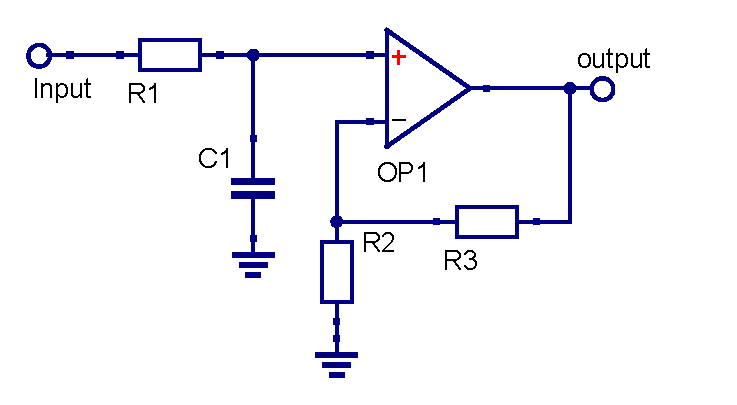
\includegraphics[width=0.5\linewidth]{pics/first-ord-lpf}
  \caption{Low-pass first order active filter section}
  \label{fig:first-ord-lpf}
\end{figure}
% \FloatBarrier

The transfer function of this section is following:
\begin{equation}
 H(s)=\frac{K_{v}C\omega_c}{s+C\omega_c}
\end{equation}

where $K_{v}$ is passband voltage gain of filter section, and $C$ is transfer
function coefficient (\ref{CN-1ord}). 

Denote by $f_c$ (Hz) the cutoff frequency:
\begin{equation}
 f_c = \frac{\omega_c}{2\pi}
\end{equation}

RC-elements values could be determined as following:
\begin{equation}
 C_1 = \frac{10}{f_c}, \quad (\mbox{uF})
\end{equation}
\begin{equation}
 R_1=\frac{1}{\omega_cC_1C}
\end{equation}
\begin{equation}
 R_2=\frac{K_vR_1}{K_v-1} \label{R2-1ord}
\end{equation}
\begin{equation}
 R_3=K_vR_1 \label{R3-1ord}
\end{equation}

For unity gain $K_v=1$ we have $R_3=0$ and $R_2=\infty$. R2 can be removed and
R3 can be shorted to obtain unity gain. 

\verb|Filter::calcFirstOrder| implements these evaluations. See
\verb|filter.cpp|.

\subsection{High pass filters}

First order section of high-pass filters circuit is shown in the Figure
\ref{fig:first-ord-lpf}

\begin{figure}[!ht]
  \centering
  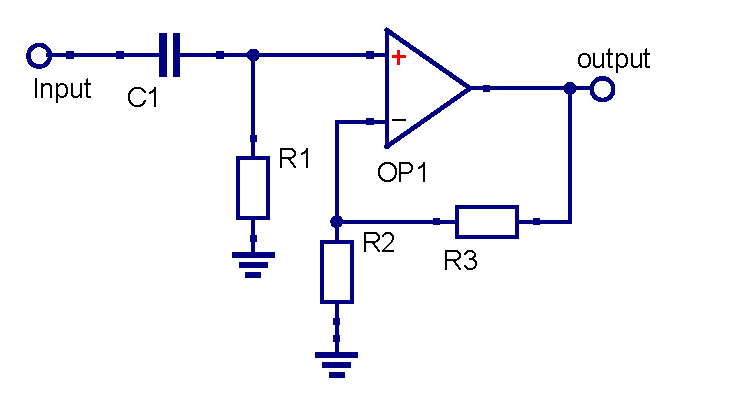
\includegraphics[width=0.5\linewidth]{pics/first-ord-hpf}
  \caption{High-pass first order active filter section}
  \label{fig:first-ord-hpf}
\end{figure}
% \FloatBarrier

Transfer function is:
\begin{equation}
 H(s)=\frac{K_v s}{s+\omega_c/C}
\end{equation}

where $C$ is transfer function coefficient (\ref{CN-1ord}).

RC-elements values could be determined as following:

\begin{equation}
 C_1 = \frac{10}{f_c}, \quad (\mbox{uF})
\end{equation}

\begin{equation}
 R_1=\frac{C}{\omega_cC_1}
\end{equation}

R2 and R3 values could be determined using equations (\ref{R2-1ord}) and
(\ref{R3-1ord}). For unity gain $K_v=1$  R2 should be removed and
R3 should be shorted. 

\verb|Filter::calcFirstOrder| implements these evaluations. This method
determines RC-elements values for both low-pass and high-pass first order
sections. See \verb|filter.cpp| for source code.

\section{Sallen-Key}

\subsection{Low pass filter}

Sallen-Key topology of low-pass filter is shown in the Figure
\ref{fig:sk-lpf}. This is second order section.

\begin{figure}[!ht]
  \centering
  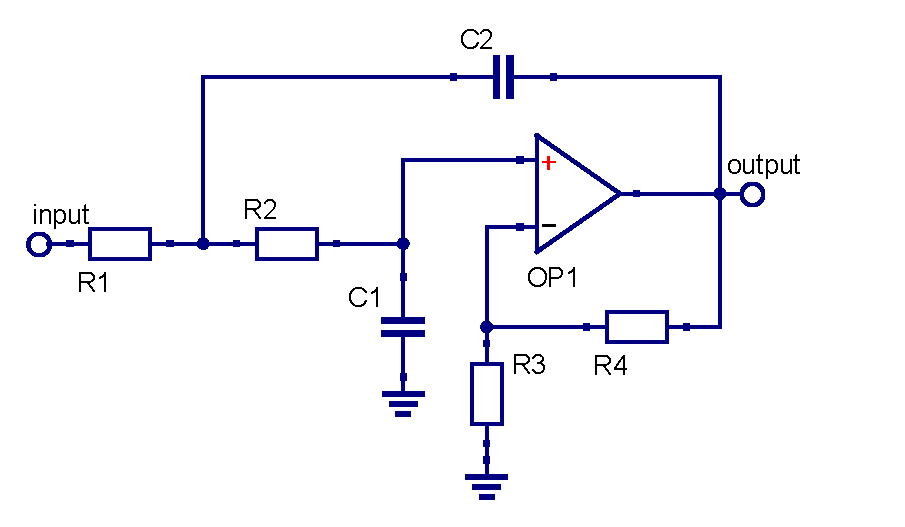
\includegraphics[width=0.6\linewidth]{pics/sk-lpf}
  \caption{Low-pass Sallen-Key active filter section}
  \label{fig:sk-lpf}
\end{figure}
% \FloatBarrier

Transfer function of Sallen-Key section has form:
\begin{equation}
 H(s)=\frac{K_v C\omega_c^2}{s^2+B\omega_cs+C\omega_c^2} \label{sk-lpf-trfunc}
\end{equation}

where $B$ and $C$ are normalized coefficient for unity cutoff frequencies
$\omega_c=1$ (\ref{Bi}), (\ref{Ci}). These coefficient could be evaluated using
poles and zeros location.

Consider Sallen-Key filter design procedure. $C_2$ capacitance could be
estimated as following:
\begin{equation}
 C_2=\frac{10}{f_c},  \quad (\mbox{uF}) \label{lp-C2}
\end{equation}

Then $C_1$ capacitance could be estimated:

\begin{equation}
 C_1\leq \frac{[B^2+4C(K_v-1)]C_2}{4C}
\end{equation}

Then we can evaluate resistors values:
\begin{equation}
 R1 = \frac{2}{\omega_c[BC_2+\sqrt{[B^2+4C(K_v-1)]C^2_2-4CC_1C_2}]}
\end{equation}

\begin{equation}
 R_2=\frac{1}{CC_1C_2R_1\omega_c^2}
\end{equation}

\begin{equation}
 R_3=\frac{K_v(R_1+R_2)}{K_v-1}
\end{equation}

\begin{equation}
 R_4=K_v(R_1+R_2)
\end{equation}

For unity gain $K_v=1$ R3 should be removed and R4 should be shorted.
\verb|SallenKey| class implements these evaluations and builds Sallen-Key
circuit. See \verb|sallenkey.cpp|.


\subsection{High pass filters}

Sallen-Key topology of high-pass filter is shown in the Figure
\ref{fig:sk-lpf}. This is second order section.

\begin{figure}[!ht]
  \centering
  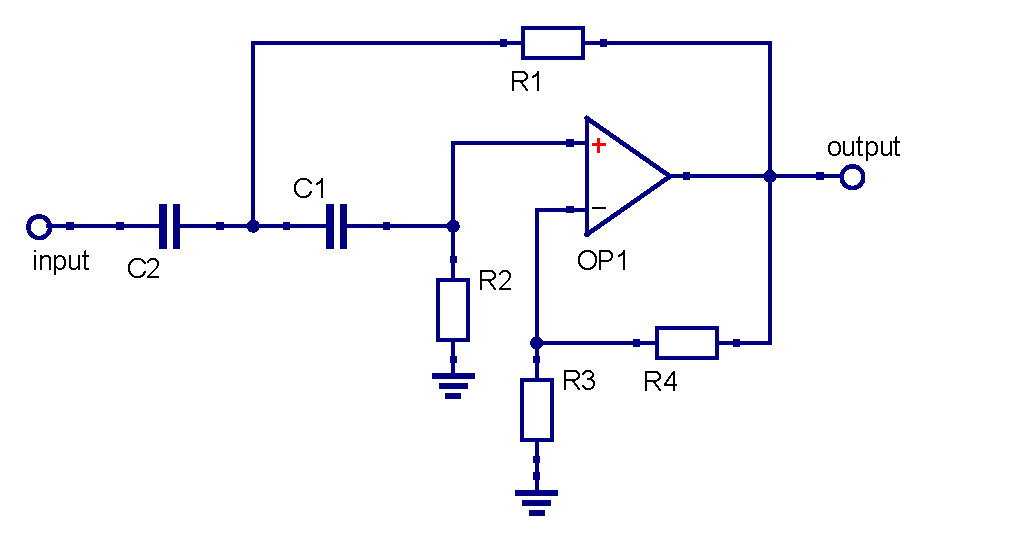
\includegraphics[width=0.6\linewidth]{pics/sk-hpf}
  \caption{High-pass Sallen-Key active filter section}
  \label{fig:sk-hpf}
\end{figure}

Transfer function of this section has the following form:
\begin{equation}
 H(s)=\frac{K_vs^2}{s^2+(B\omega_c/C)s+\omega_c^2/C} \label{sk-hpf-trfunc}
\end{equation}

where $B$ and $C$ are normalized coefficients of the low-pass prototype filter.
These coefficients could be evaluated using poles and zeros location of the
low-pass prototype.

RC-elements values evaluation methods are similar to low-pass section. C1 and
C2 capacitors values are equals:
\begin{equation}
 C_1=C_2=\frac{10}{f_c}, \quad (\mbox{uF})
\end{equation}

Then we can evaluate resistors values:
\begin{equation}
 R_2=\frac{4C}{[B+\sqrt{B^2+8C(K_v-1)}]\omega_cC_1}
\end{equation}
\begin{equation}
 R_1=\frac{C}{\omega_c^2C_1^2R_2}
\end{equation}
\begin{equation}
 R_3=\frac{K_vR_2}{k_v-1}
\end{equation}
\begin{equation}
 R_4=K_vR_2
\end{equation}


For unity gain $K_v=1$ R3 should be removed and R4 should be shorted.
\verb|SallenKey| class implements these evaluations and builds Sallen-Key
circuit. See \verb|sallenkey.cpp|.

\subsection{Band pass filter}

Sallen-Key topology of abnd-pass filter is shown in the Figure
\ref{fig:sk-bpf}. Two such section should be connected in series to implement
2-nd order section of band-pass filter.

\begin{figure}[!ht]
  \centering
  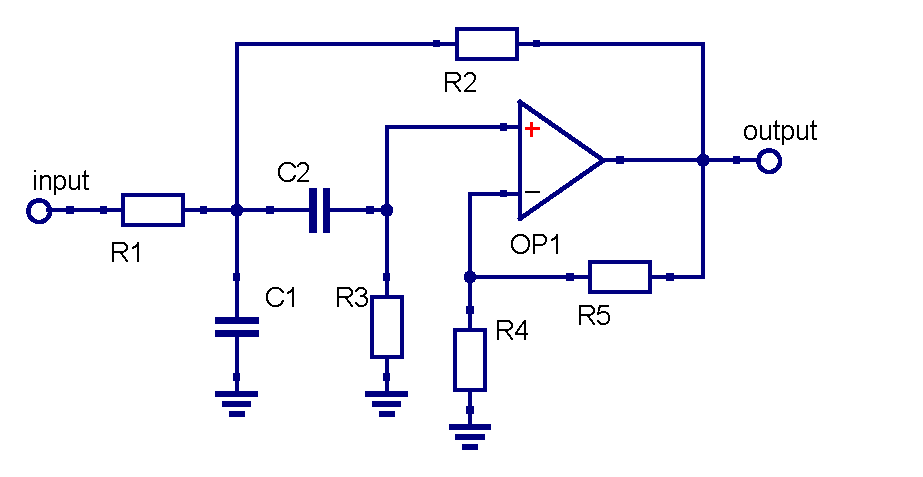
\includegraphics[width=0.6\linewidth]{pics/sk-bpf}
  \caption{Band pass Sallen-Key active filter section}
  \label{fig:sk-bpf}
\end{figure}
%\FloatBarrier

Transfer function of this topology is:
\begin{equation}
 H(s) = \frac{\rho\omega_0}{s^2+\beta\omega_0s+\gamma\omega_0^2} 
\label{eq:sk-bpf-trfunc}
\end{equation}

where $\rho$, $\beta$, $\gamma$  are some coefficients. These coefficients 
depend on RC-elements values.


Using this topology we can implement three types of filter sections:

\begin{enumerate}
 \item Second order band-pass filter
 \item Second-order (Chebyshev, Butterworth, or Cauer) band-pass filter section 
that corresponds second-order section of an LPF prototype.
 \item Second-order band-pass filter section that corresponds first-order 
section of an LPF prototype.
\end{enumerate}

To calculate such section at first we should determine $\rho$, $\beta$, 
$\gamma$ coefficients. The will be following.

\begin{itemize}
 \item For second order band-pass filter
 \begin{equation}
  \rho = \frac{K_{v}}{Q}
 \qquad
  \beta = \frac{1}{Q}
\qquad
  \gamma = 1.0
 \end{equation}

 \item For second-order (Chebyshev, Butterworth, or Cauer) band-pass filter 
section that corresponds second-order section of an LPF prototype. At first 
coefficients $B_i$ and $C_i$ should be evaluated from poles and zeros set of 
low-pass prototype using (\ref{Bi}) and (\ref{Ci}). Then supplementary 
coefficient $D$, $E$, $F$, $H$ should be calculated for every section of the 
filter. 

\begin{equation}
 H = C+ 4Q^2
\end{equation}
\begin{equation}
 E = \frac{1}{B}\sqrt{\frac{(H+\sqrt{H^2-4B^2Q^2})}{2}}
\end{equation}
\begin{equation}
 F=\frac{BE}{Q}
\end{equation}
\begin{equation}
 D = \frac{F+\sqrt{F^2-4}}{2}
\end{equation}

After this evaluation is performed we can evaluate $\rho$, $\beta$, $\gamma$ 
coefficients. Second order section of band-pass filter consists of two 
sections. For first section coefficients are:

\begin{equation}
 \rho = \frac{K_v\sqrt{C}}{Q}
\end{equation}

\begin{equation}
 \beta = D/E
\end{equation}
\begin{equation}
 \gamma = D^2
\end{equation}

And for second section:

\begin{equation}
 \rho = \frac{K_v\sqrt{C}}{Q}
\end{equation}

\begin{equation}
 \beta = \frac{1}{DE}
\end{equation}
\begin{equation}
 \gamma = \frac{1}{D^2}
\end{equation}

\item For second-order band-pass filter section that corresponds first-order 
section of an LPF prototype. We need to calculate coefficient $C_i$ from filter 
poles. Coefficients are:

\begin{equation}
 \rho=\frac{K_v C}{Q}
\qquad
 \beta = \frac{C}{Q}
\qquad
 \gamma=1.0
\end{equation}

\end{itemize}

Having $\rho$, $\beta$, $\gamma$ coefficients we can calculate RC-elements 
values:

\begin{equation}
 C_1=C_2=\frac{10.0}{2\pi\omega_0}\qquad(\mbox{uF})
\end{equation}
\begin{equation}
 R_1 = \frac{2}{\rho\omega_0C_1}
\end{equation}
\begin{equation}
 R_2=\frac{2}{-\beta+\sqrt{[(\rho-\beta)^2+8\gamma]\omega_0C_1}}
\end{equation}
\begin{equation}
 R_3 = 
\frac{1}{\gamma\omega_0^2C_1^2}\cdot\left(\frac{1}{R_1}+\frac{1}{R_2}\right)
\end{equation}
\begin{equation}
 R_4=2R_3
\end{equation}

Now we can substitute RC-elements values and build filter circuit. 
\verb|SallenKey::calcBandPass()| implements these calculations. See 
\verb|sallenkey.cpp|


\section{Multifeedback}

\subsection{Low pass filter}

Multifeedback (MFB) circuit of low-pass filter is shown in the Figure
\ref{fig:mfb-lpf}. 

\begin{figure}[!ht]
  \centering
  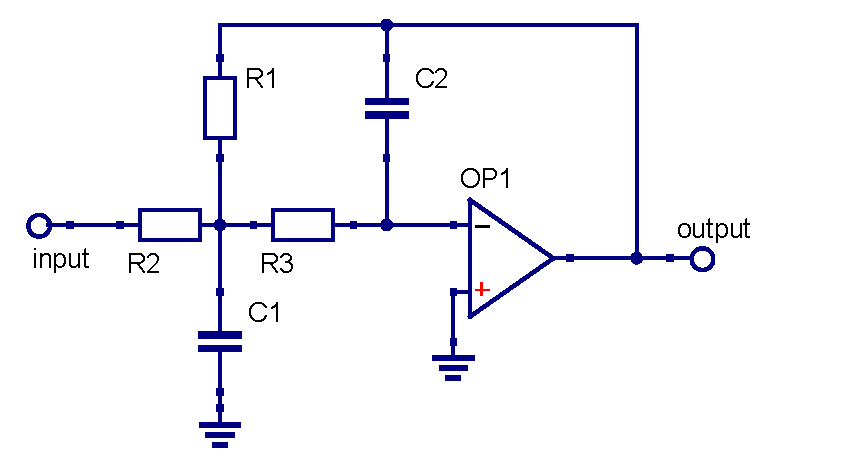
\includegraphics[width=0.6\linewidth]{pics/mfb-lpf}
  \caption{Low-pass multifeedback active filter section}
  \label{fig:mfb-lpf}
\end{figure}
% \FloatBarrier

Transfer function of this section has form (\ref{sk-lpf-trfunc}). Having
normalized transfer function coefficients $B$ and $C$ we can determine
RC-elements values. At first, select $C_2$ using equation (\ref{lp-C2}). Then
we can determine $C_1$ value
\begin{equation}
 C_1\leq\frac{B^2C_2}{4C(K_v+1)}
\end{equation}

Using $C_1$ and $C_2$ we can determine resistors values
\begin{equation}
 R_2=\frac{2(K_v+1)}{[BC_2+\sqrt{B^2C_2^2-4CC_1C_2(K_v+1)}]\omega_c}
\end{equation}
\begin{equation}
 R_1=\frac{R_2}{K_v}
\end{equation}
\begin{equation}
 R_3=\frac{1}{CC_1C_2\omega_c^2R_2}
\end{equation}

\verb|MFBfilter| class is responsible for multifeedback filter circuit
calculation and building. \verb|MFBfilter::calcLowPass()| method evaluates
RC-elements values. 

\verb|MFBfilter::createLowPassSchematic()| method builds
low-pass filter schematic for Qucs. See \verb|mfbfilter.cpp| for source code.




\subsection{High pass filters}

Multifeedback (MFB) circuit of low-pass filter is shown in the Figure
\ref{fig:mfb-hpf}. 

\begin{figure}[!ht]
  \centering
  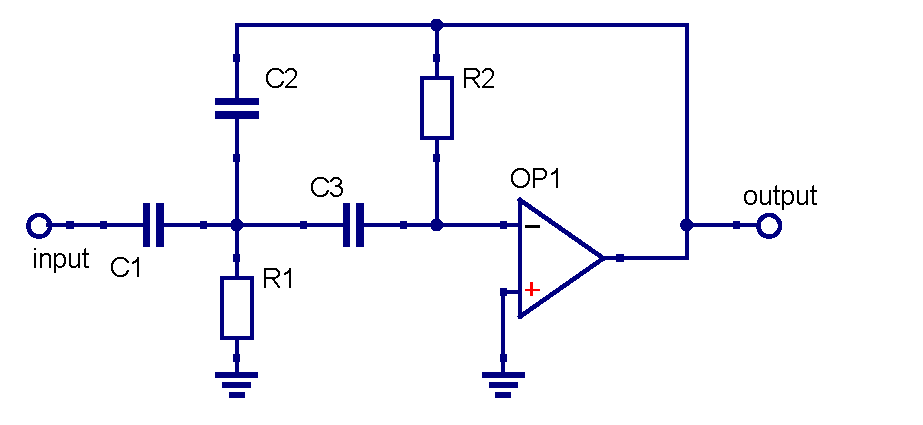
\includegraphics[width=0.6\linewidth]{pics/mfb-hpf}
  \caption{Low-pass multifeedback active filter section}
  \label{fig:mfb-hpf}
\end{figure}
% \FloatBarrier

Transfer function of this section has form (\ref{sk-hpf-trfunc}). 

RC-elements value could be evaluated as following:

\begin{equation}
 C_1=C_3=\frac{10}{f_c}
\end{equation}
\begin{equation}
 C_2=\frac{C_1}{K_v}
\end{equation}
\begin{equation}
 R_1=\frac{B}{\omega_c(2C_1+C_2)}
\end{equation}
\begin{equation}
 R_2=\frac{(2C_1+C_2)C}{BC_1C_2\omega_c}
\end{equation}

\verb|MFBfilter::calcHighPass()| and \verb|MFBfilter::createHighPassSchematic()|
methods are responsible for multifeedback high-pass filter design. See
\verb|mfbfilter.cpp|

\subsection{Band pass filter}

MFB band-pass filter section topology is shown in the Figure \ref{fig:mfb-bpf}.

\begin{figure}[!ht]
  \centering
  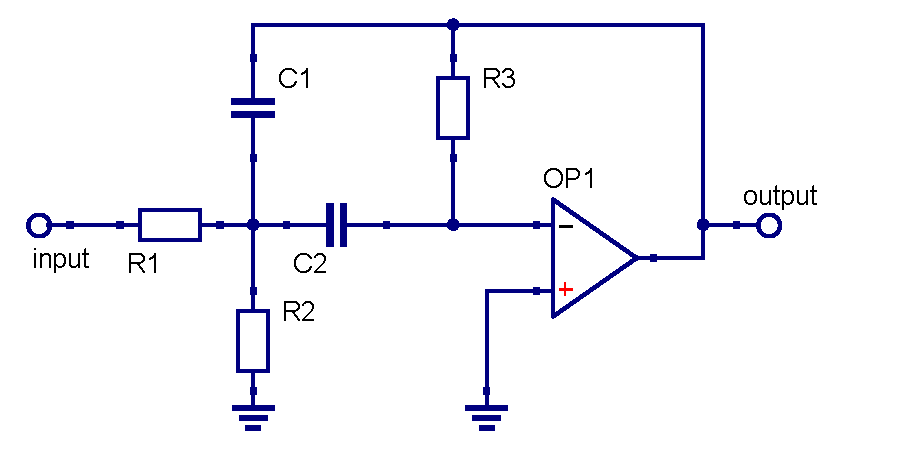
\includegraphics[width=0.6\linewidth]{pics/mfb-bpf}
  \caption{Band pass multifeedback active filter section}
  \label{fig:mfb-bpf}
\end{figure}
% \FloatBarrier

This section has transfer function of the form (\ref{eq:sk-bpf-trfunc}). It is 
need to determine $\rho$, $\beta$, $\gamma$ coefficients set using method 
presented in previous section. Having these coefficients we can evaluate 
RC-elements values. 

\begin{equation}
 C_1=\frac{10.0}{2\pi\omega_0}\qquad(\mbox{uF})
\end{equation}

\begin{equation}
 C_2 = \frac{C_1(\rho\beta-\gamma)}{\gamma}
\end{equation}

If $C_2$ is less than zero ($C_2<0$) we should put $C_2=C_1$.

\begin{equation}
 R_1 = \frac{1}{\rho\omega_0}
\end{equation}
\begin{equation}
 R_2=\frac{\beta}{[C_1(\gamma-\rho\beta)+\gamma C_2]\omega_0}
\end{equation}
\begin{equation}
 R_3=\frac{1}{\beta\omega_0}\left(\frac{1}{C_1}+\frac{1}{C_2}\right)
\end{equation}

Now we can substitute RC-elements values and build filter circuit. 
\verb|MFBfilter::calcBandPass()| implements these calculations. See 
\verb|mfbfilter.cpp|




\section{Cauer and Chebyshev Type-II filters}

\subsection{Low pass filter}

Low-pass Cauer filter schematic is shown in the Figure \ref{fig:sch_cauer}.
High-pass section of Cauer filter has the same topology.

\begin{figure}[!ht]
  \centering
  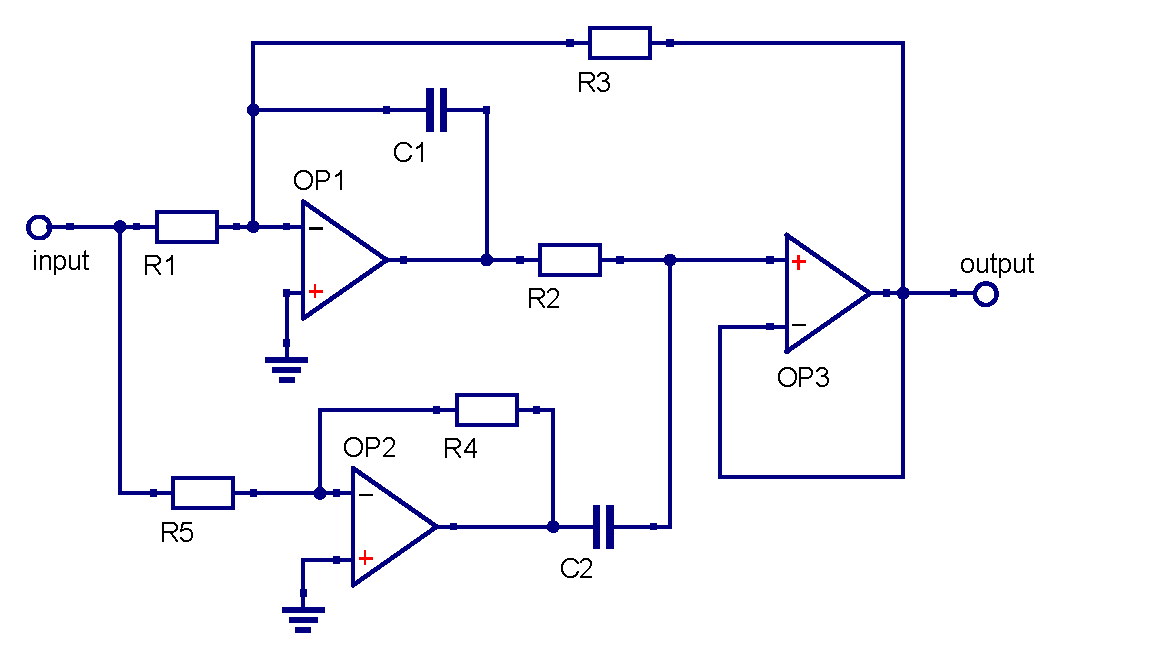
\includegraphics[width=0.8\linewidth]{pics/cauer}
  \caption{Low-pass and high-pass Cauer active filter section}
  \label{fig:sch_cauer}
\end{figure}
% \FloatBarrier

We should know $A_i$, $B_i$, and $C_i$ transfer function coefficients to
evaluate RC-elements values of the Cauer filter.

Capacitors values are:

\begin{equation}
 C_1=C_2=\frac{10}{f_c} \qquad \mbox{(uF)}  \label{eq:cauer_C1_C2}
\end{equation}

Resistors values are:

\begin{equation}
 R_5=\frac{1}{\omega_c C_1} \label{eq:cauer_R5}
\end{equation}
\begin{equation}
 R_1=\frac{BR_5}{K_v C}
\end{equation}
\begin{equation}
 R_2=\frac{R_5}{B}
\end{equation}
\begin{equation}
 R_3=\frac{BR_5}{C}
\end{equation}
\begin{equation}
 R_4=\frac{K_v C R_5}{A}
\end{equation}

\verb|SchCauer::calcLowPass()| and \verb|SchCauer::createLowPassSchematic()|
methods implement these evaluation. See \verb|schcauer.cpp|



\subsection{High pass filters}

High-pass section of Cauer filters use the same topology as low-pass section
(\ref{fig:sch_cauer}). Capacitors values could be determined using equation
(\ref{eq:cauer_C1_C2}). R5 resistors value using (\ref{eq:cauer_R5})

\begin{equation}
 R_1 = \frac{A B R_5}{K_v C}
\end{equation}
\begin{equation}
 R_2 = \frac{C R_5}{B}
\end{equation}
\begin{equation}
 R_3=B R_5
\end{equation}
\begin{equation}
 R_4 = K_v R_5
\end{equation}

\verb|SchCauer::calcHighPass()| and \verb|SchCauer::createHighPassSchematic()|
methods implement these evaluation. See \verb|schcauer.cpp|


\subsection{Band pass filters}

The topology of Cauer band-pass filter differs from LPF and HPF topology. 
Schematic is presented in the Figure \ref{fig:sch_bandpass}. There are two 
additional resistors R6 and R7.

\begin{figure}[!ht]
  \centering
  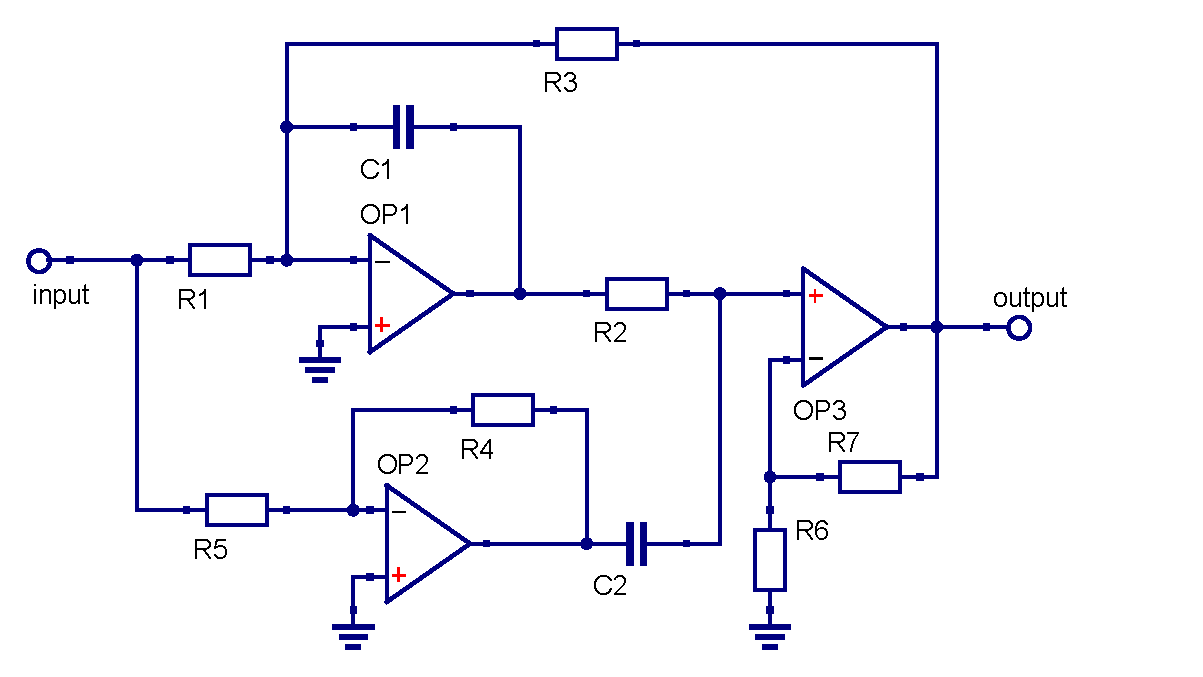
\includegraphics[width=0.8\linewidth]{pics/cauer-bandpass}
  \caption{Low-pass and high-pass Cauer active filter section}
  \label{fig:sch_bandpass}
\end{figure}
% \FloatBarrier

Transfer function of such section has the following form:
\begin{equation}
 H(s) = \frac{\rho(s^2+\alpha\omega_0^2)}{s^2+\beta\omega_0s+\gamma\omega_0^2}
\end{equation}


At first we need to determine $A_i$, $B_i$, $C_i$ coefficients set (\ref{Ai}), 
(\ref{Bi}), and (\ref{Ci}) for every section of the filter. Qucs-activefilter 
build schematic only for even order prototype of Cauer band-pass filters. If 
low-pass prototype has odd order, then order is expanded to nearest even order.

It's need to evaluate the following coefficients for every $i$-th section of 
the low-pass prototype:

\begin{equation}
 A_1 = 1+\frac{A+\sqrt{A^2+4AQ^2}}{2Q^2}
\end{equation}
\begin{equation}
 H=C+4Q^2
\end{equation}
\begin{equation}
 E=\frac{1}{B}\sqrt{\frac{H+\sqrt{H^2-4B^2Q^2}}{2}}
\end{equation}
\begin{equation}
 F=\frac{BE}{Q}
\end{equation}
\begin{equation}
 D=\frac{F+\sqrt{F^2-4}}{2}
\end{equation}

Let $\mu$ be $\mu=2.0$.

Second order section of low-pass prototype corresponds two second-order 
sections of band-pass filter. Capacitors values for these sections are equals. 

\begin{equation}
 C1 = C2 = \frac{20\pi}{\omega_0} \qquad (uF) \label{eq:C1_C2_bpf}
\end{equation}

Resistors values for the first section:
\begin{equation}
 R_1= \frac{\mu D}{K_v A_1 E \omega_0 C_1}\cdot\sqrt{\frac{A}{C}}
\end{equation}
\begin{equation}
 R_2=\frac{E}{DE\omega_0 C_2}
\end{equation}
\begin{equation}
 R_3=\frac{\mu}{DE\omega_0 C_1}
\end{equation}

For the second section:
\begin{equation}
 R_1= \frac{\mu A_1}{K_v D E \omega_0 C_1}\cdot\sqrt{\frac{A}{C}}
\end{equation}
\begin{equation}
 R_2=\frac{DE}{\omega_0 C_2}
\end{equation}
\begin{equation}
 R_3=\frac{\mu D}{E\omega_0 C_1}
\end{equation}

For both sections:
\begin{equation}
 R_5=R_3
\end{equation}
\begin{equation}
 R_4=\frac{K_v R_5}{\mu}\cdot\sqrt{\frac{C}{A}}
\end{equation}
\begin{equation}
 R_6=\frac{\mu R_2}{\mu - 1}
\end{equation}
\begin{equation}
 R_7 = \mu R_2
\end{equation}


Now we can substitute RC-elements values and build filter circuit. 
\verb|SchCauer::calcBandPass()| implements these calculations. See 
\verb|schcauer.cpp|




\section{Band stop filters}


Band stop filter can be implemented using Cauer active filter section topology 
for band-pass filters (Figure \ref{fig:sch_bandpass}).

Transfer function of such section has the following form:
\begin{equation}
 H(s) = \frac{\rho(s^2+\alpha\omega_0^2)}{s^2+\beta\omega_0s+\gamma\omega_0^2}
\end{equation}

At first, we need to evaluate some coefficients for every section of low-pass 
prototype. These coefficients should be found using $A_i$, $B_i$, $C_i$ 
coefficients, that could be found from poles and zeros of low-pass prototype 
transfer function.

For Cauer or Chebyshev Type-II coefficient $A_2$:
\begin{equation}
 A_2 = 1+\frac{1+\sqrt{1+4AQ^2}}{2AQ^2}
\end{equation}

For Butterworth, Chebyshev Type-I, or Bessel filters we should put $A_2=1$. Let 
$\mu$ be $\mu=2.0$.

Other coefficients:
\begin{equation}
 H = 1+4CQ^2
\end{equation}
\begin{equation}
 E_1=\frac{1}{B}\sqrt{\frac{C(H+\sqrt{H^2-4B^2Q^2})}{2}}
\end{equation}
\begin{equation}
 G=\frac{BE_1}{QC}
\end{equation}
\begin{equation}
 D_1=\frac{G+\sqrt{G^2-4}}{2}
\end{equation}

For the first section:
\begin{equation}
 \alpha = A_2 \qquad \beta=\frac{D_1}{E_1} \qquad \gamma=G^2
\end{equation}


For the second section:
\begin{equation}
 \alpha = \frac{1}{A_2} \qquad \beta=\frac{1}{D_1E_1} \qquad 
\gamma=\frac{1}{G^2}
\end{equation}

Capacitors values should be evaluated using (\ref{eq:C1_C2_bpf}). Resistors 
values for first section are:
\begin{equation}
R_1=\frac{\mu\beta}{K_v\alpha\omega_0C_1} 
\end{equation}
\begin{equation}
 R_2=\frac{1}{\beta\omega_0 C_2}
\end{equation}
\begin{equation}
 R_3=\frac{K_v\alpha R_1}{\gamma}
\end{equation}
\begin{equation}
 R_5 = \frac{1}{\omega_0 C_1}
\end{equation}
\begin{equation}
 R_4=\frac{K_vR_5}{\mu}
\end{equation}
\begin{equation}
 R_6=R_7=\frac{\mu R_2}{\mu-1}
\end{equation}


Now we can substitute RC-elements values and build filter circuit. 
\verb|SchCauer::calcBandStop()| implements these calculations. See 
\verb|schcauer.cpp|


\chapter{Conclusion}

Qucsactivefilter is powerful tool that allows you to build filter circuits. The 
following filter topologies are implemented:
\begin{enumerate}
 \item Sallen-Key low-pass, high-pass, and band-pass filters. Butterworth, 
Chebyshev Type-I, and Bessel approximations.
 \item Multifeedback low-pass, high-pass, and band-pass filters. Butterworth, 
Chebyshev Type-I, and Bessel approximations.
 \item Cauer low-pass, high-pass, and band-pass filters. Chebyshev Type-II and 
Cauer approximations.
 \item Cauer band-stop filters. Butterworth, Chebyshev Type-I, Bessel, and 
Cauer approximations.
 \item User defined transform function approximation --- all types of filter 
topologies.
\end{enumerate}

Background mathematics filter synthesis methods were considered. These methods 
are used in Qucsactivefilter sources. 

You can implement physical filters after filter circuit is built and simulated 
with Qucs. It's need to note that real RC-elements values have tolerances. You 
should use RC-elements with at at least less than 1\% tolerance. Filter circuit 
may require RC-elements values trimming. For trimming methods see 
\cite {johnson} and \cite{Moschytz}. 


\bibliographystyle{IEEEtran}
\bibliography{activefilter}


